\documentclass[12pt]{article}

% Cabeçalho e formatação adaptados de Meio ambiente/Ensaio 1/Ensaio-1_Gabriel_Cintra.tex.
\usepackage[T1]{fontenc}
\usepackage[utf8]{inputenc}
\usepackage[brazilian]{babel}
\usepackage{microtype}
\usepackage{geometry}
\geometry{a4paper, margin=2.5cm}
\usepackage{parskip}
\usepackage{graphicx}
\usepackage{hyperref}
\hypersetup{colorlinks=true, urlcolor=blue, linkcolor=blue, citecolor=blue}

\newcommand{\instituicao}{UNIVERSIDADE FEDERAL DE SANTA CATARINA}
\newcommand{\departamento}{Programa de Pós-Graduação em Economia}
\newcommand{\curso}{Mestrado}
\newcommand{\disciplina}{Desigualdade, Diversidade e Redes}
\newcommand{\titulo}{Rede intersetorial de emissões no Brasil}
\newcommand{\subtitulo}{Relatório de análise exploratória}
\newcommand{\autor}{Gabriel Pincelli Cintra}
\newcommand{\local}{Florianópolis}
\newcommand{\dataentrega}{\today}

% Cabeçalho na primeira página, sem capa.
\newcommand{\imprimirtitulodois}{
\begin{center}
  {\Large\bfseries\MakeUppercase{\instituicao}\par}
  \vspace{0.2em}
  {\large \departamento\par}
  \vspace{0.2em}
  {\normalsize\textbf{\disciplina}\ (\curso)\par}
  \vspace{1.4em}
  {\LARGE\bfseries \titulo\par}
  \vspace{0.25em}
  {\large\itshape \subtitulo\par}
  \vspace{1.5em}
\end{center}
\noindent
\begin{minipage}{0.48\textwidth}
  \raggedright\normalsize \autor
\end{minipage}\hfill
\begin{minipage}{0.48\textwidth}
  \raggedleft\normalsize \local, \dataentrega
\end{minipage}
\vspace{1.0em}
\hrule
\vspace{1.0em}
}

\begin{document}
\imprimirtitulodois
% Texto principal reproduzido do README, sem revisão editorial.
Os processos produtivos geram externalidades ambientais. A percepção geral é de que os níveis atuais de produção são insustentáveis e de que estamos caminhando para mudanças climáticas irreversíveis (\href{https://doi.org/10.1126/science.abn7950}{Armstrong McKay et al., 2022}).

Entre essas externalidades, as emissões de dióxido de carbono (CO\textsubscript{2}) ocupam posição central no debate sobre mudanças climáticas e constituem o foco deste ensaio.

Para poder controlar as emissões e mitigar seus efeitos, é essencial que possamos quantificá-las de forma a atribuir responsabilidades aos agentes econômicos envolvidos (\href{https://doi.org/10.1016/j.ecolecon.2012.09.010}{Marques et al., 2012}).

Há ampla discussão sobre os critérios utilizados para mensurar as emissões e atribuir responsabilidade aos agentes econômicos envolvidos. A metologia estabelecida no protocolo de Kyoto (\href{https://unfccc.int/resource/docs/publications/08_unfccc_kp_ref_manual.pdf}{UNFCCC, 2008}) é amplamente utilizada e atribui a responsabilidade ao território onde as emissões foram realizadas.

Diversos estudos foram feitos para contabilizar as emissões brasileiras, incluindo trabalhos recentes de \href{https://doi.org/10.1016/j.rspp.2024.100015}{Sanguinet e Azzoni (2024)} e \href{https://doi.org/10.1007/s10668-024-05251-8}{Montoya et al. (2026)}. Esses estudos permitem identificar os setores responsáveis pelos maiores volumes de emissões, mas não evidenciam a estrutura das relações intersetoriais associadas a essas emissões.

O presente ensaio propõe uma análise de redes para explorar a estrutura intersetorial das emissões atribuídas à produção brasileira. A análise busca identificar não apenas quais setores concentram os maiores volumes de emissões, mas também como essas emissões se distribuem ao longo da cadeia produtiva.

A primeira hipótese é de que os setores com maiores níveis de emissões estejam amplamente conectados à estrutura produtiva.

A segunda hipótese é de que existam setores com baixos níveis de emissões diretas, mas cuja produção dependa de insumos provenientes de múltiplos setores intensivos em emissões.

A rede será construída a partir da MIP 2015, nível 67 (\href{https://www.ibge.gov.br/estatisticas/economicas/contas-nacionais/9085-matriz-de-insumo-produto.html}{IBGE}), utilizando coeficientes de emissão propostos por \href{https://doi.org/10.1016/j.rspp.2024.100015}{Sanguinet e Azzoni (2024)} e adotando a abordagem de responsabilidade baseada na produção discutida por \href{https://doi.org/10.1016/j.ecolecon.2012.09.010}{Marques et al. (2012)} e adotada no protocolo de Kyoto (\href{https://unfccc.int/resource/docs/publications/08_unfccc_kp_ref_manual.pdf}{UNFCCC, 2008}). As relações entre os setores serão representadas por uma rede ponderada pelos volumes de emissões atribuídos às relações intersetoriais. A análise será feita em Python, utilizando a biblioteca NetworkX. O código-fonte e os resultados serão disponibilizados no \href{https://github.com/G-Cintra/Redes}{repositório do projeto}.

A partir dos resultados, serão discutidas possíveis implicações para políticas públicas e tecnologias de mitigação, considerando as propostas apresentadas por \href{https://doi.org/10.1016/j.apenergy.2020.114848}{Rissman et al. (2020)}.

\section*{Acompanhamento da análise}
Repositório: \url{https://github.com/G-Cintra/Redes/}

Página de resultados: \url{https://g-cintra.github.io/Redes/}

As quatro figuras seguintes reproduzem as primeiras visualizações da página, na mesma ordem. Os resultados são preliminares e exploratórios; as definições e hipóteses metodológicas estão no README do repositório.

\clearpage
\begin{figure}[p]
\centering
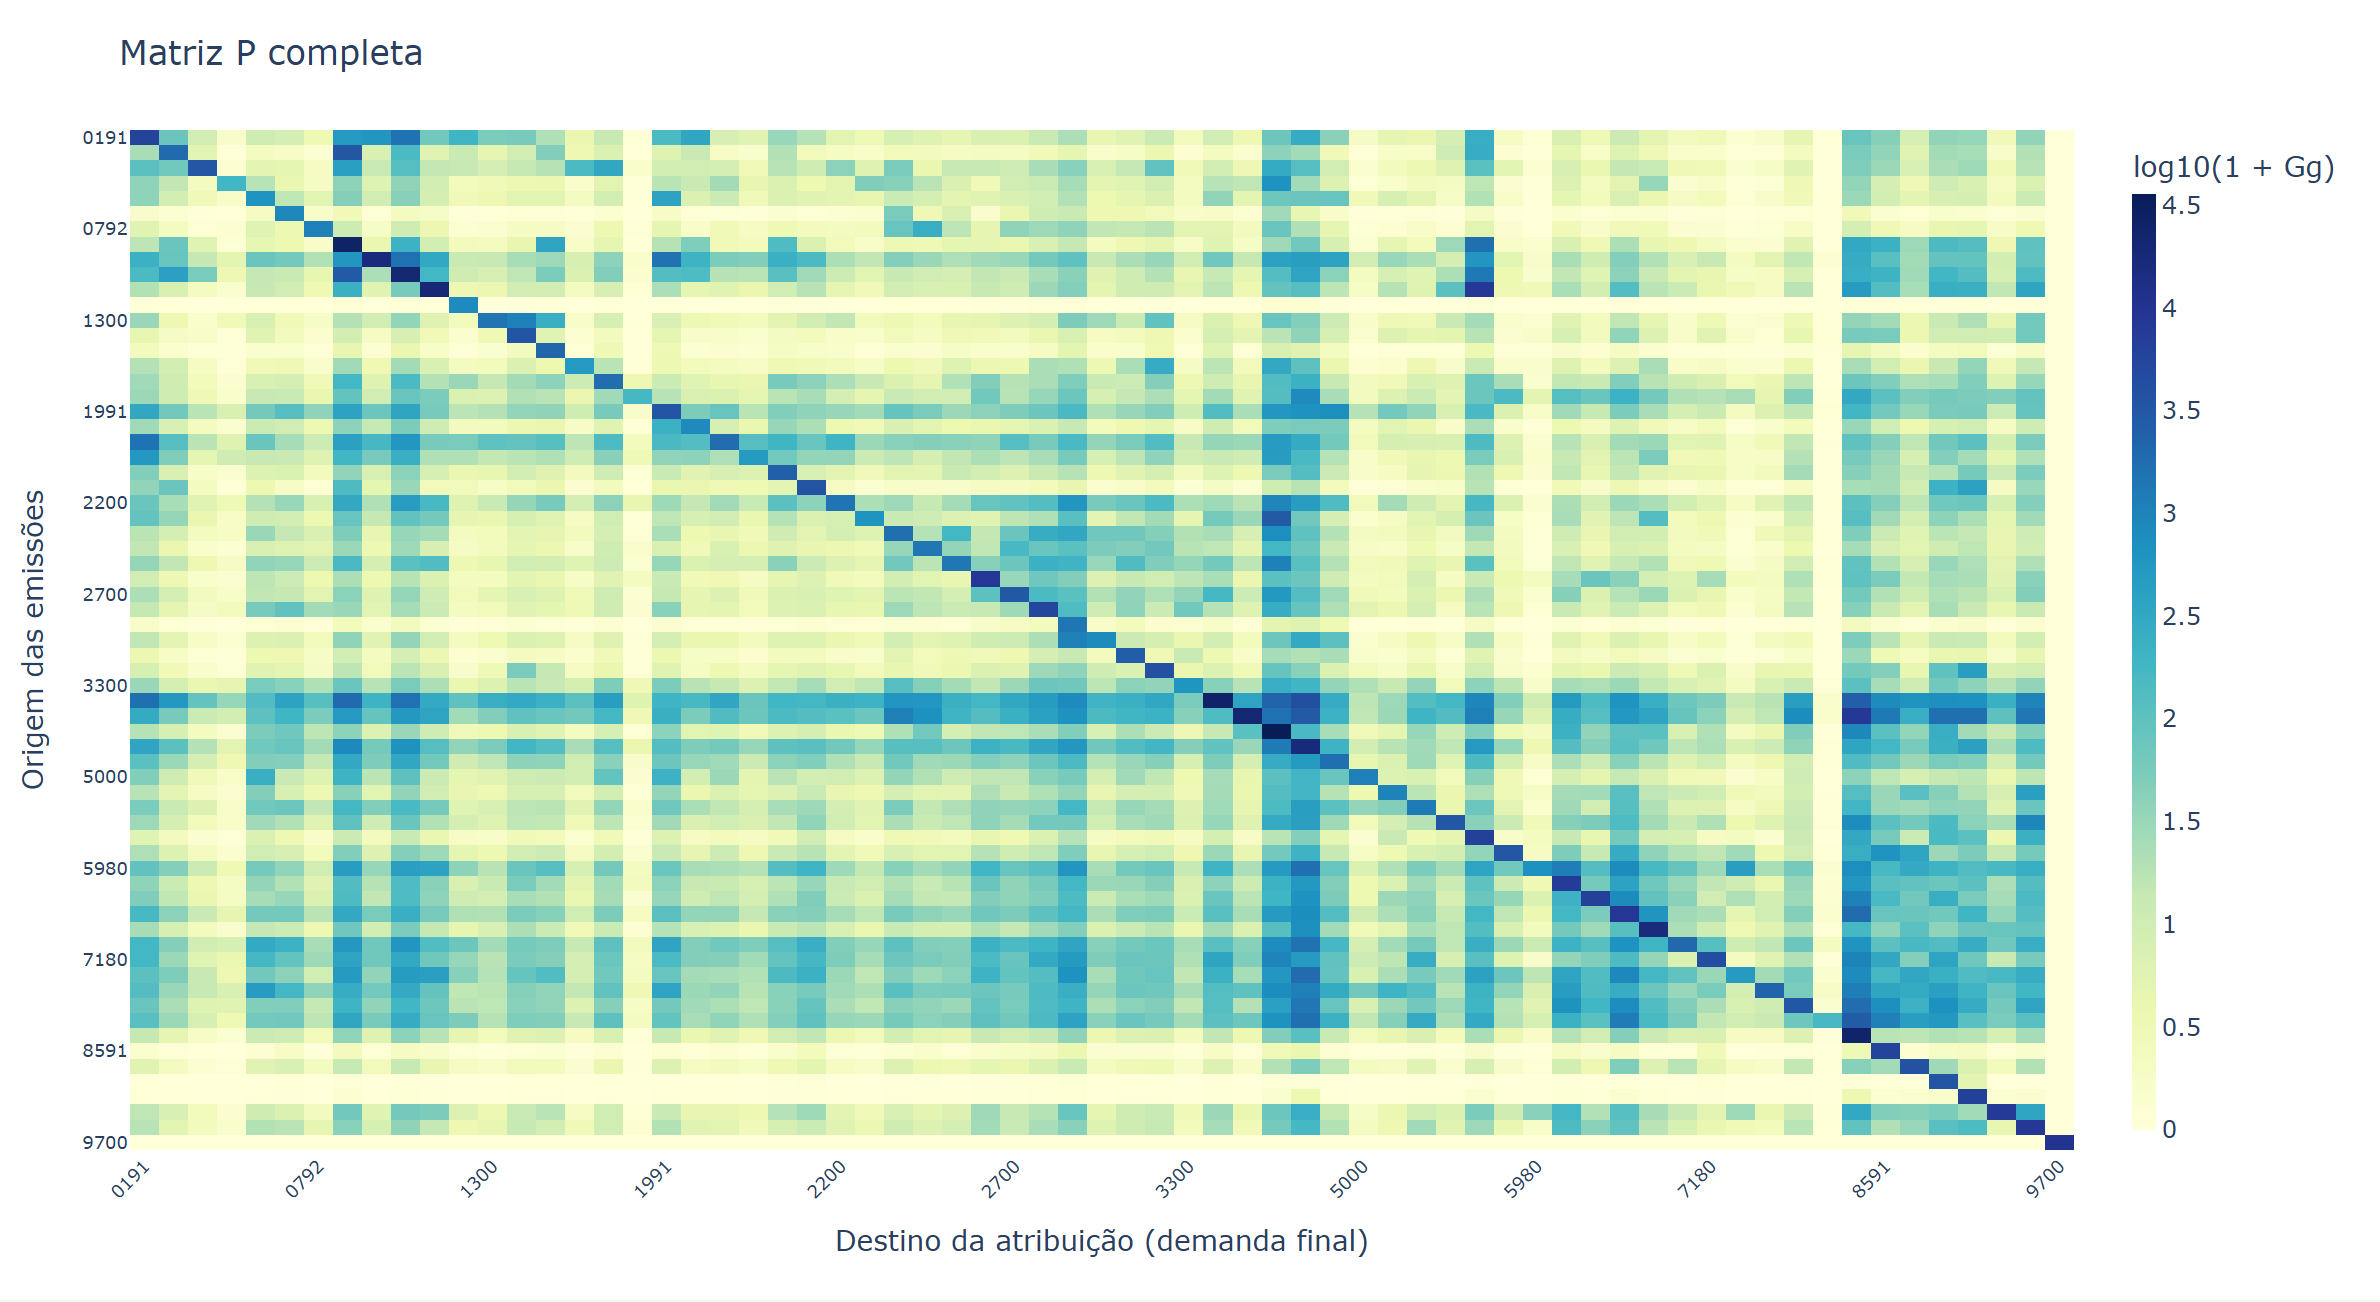
\includegraphics[width=\textwidth,height=0.87\textheight,keepaspectratio]{imagens/01_matriz_p.png}
\caption{Matriz P: heatmap. As linhas identificam as atividades emissoras e as colunas, os destinos da demanda final. A diagonal reúne as atribuições à própria atividade. A cor representa a escala logarítmica indicada no gráfico.}
\end{figure}

\clearpage
\begin{figure}[p]
\centering
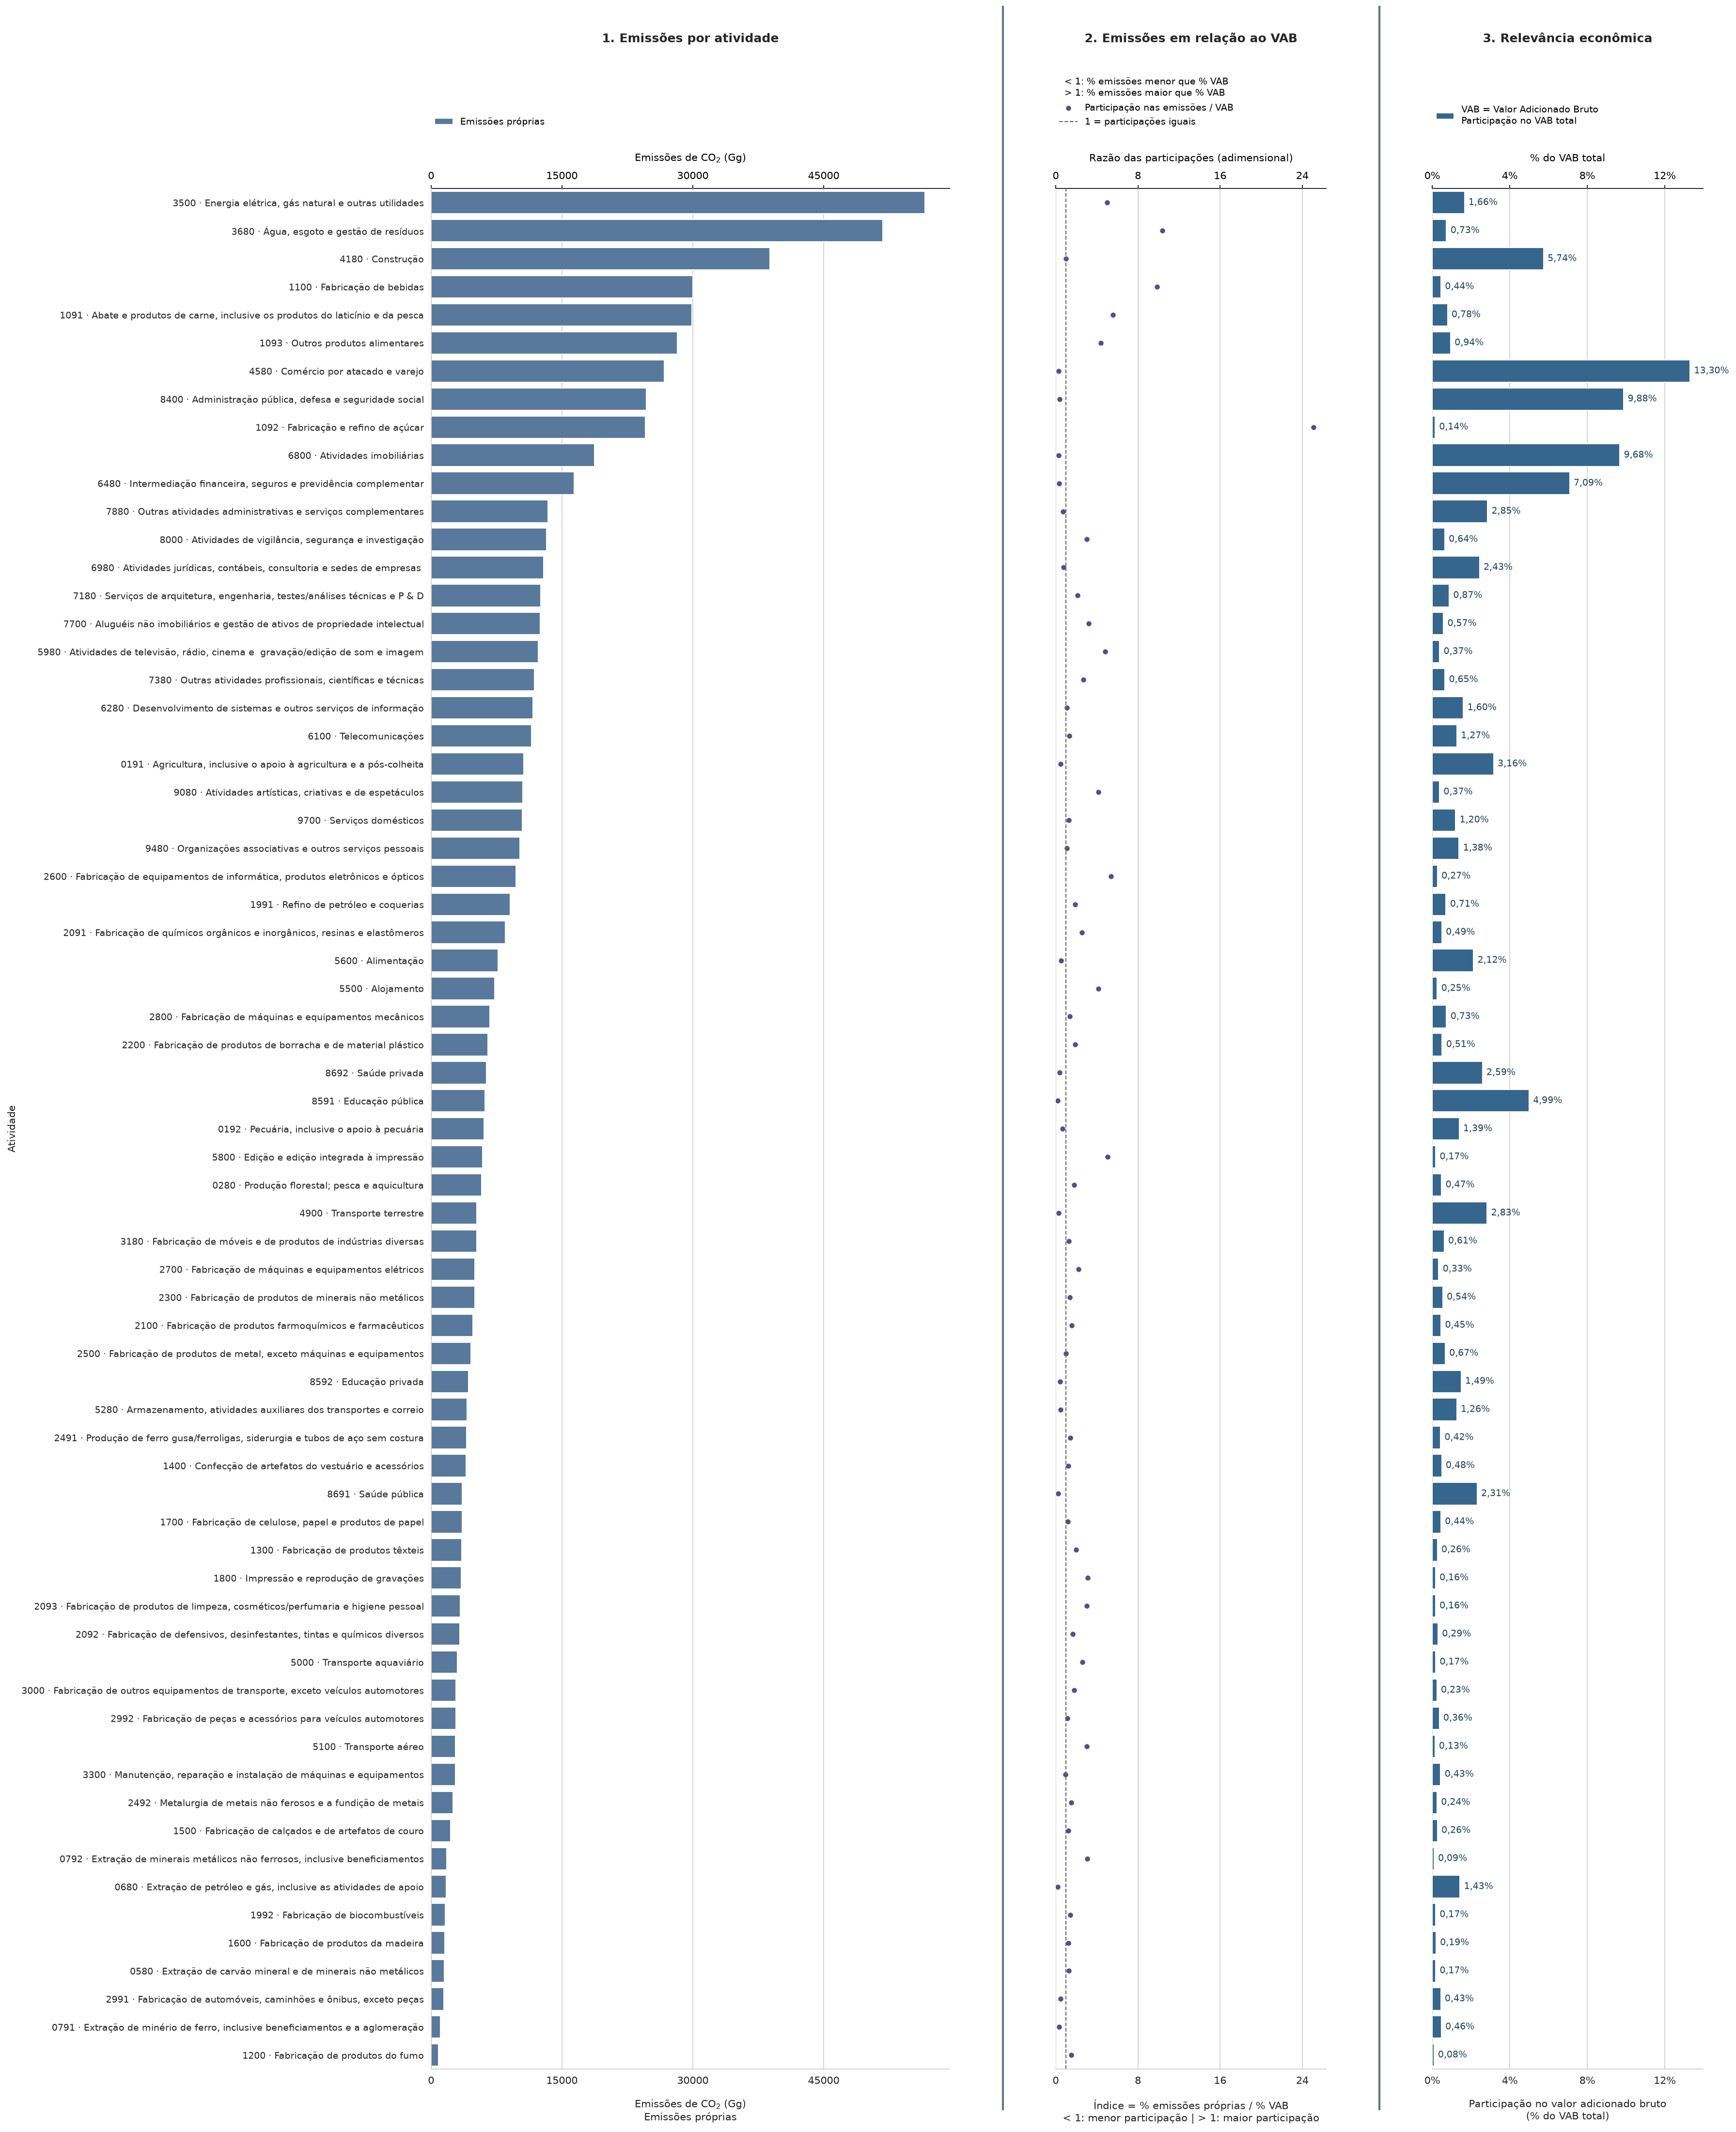
\includegraphics[width=\textwidth,height=0.87\textheight,keepaspectratio]{imagens/02_emissoes_vab.png}
\caption{Emissões próprias e participação no valor adicionado bruto. Os três painéis mostram emissões próprias, razão entre participações nas emissões e no VAB, e participação no VAB. As atividades estão ordenadas pelas emissões próprias.}
\end{figure}

\clearpage
\begin{figure}[p]
\centering
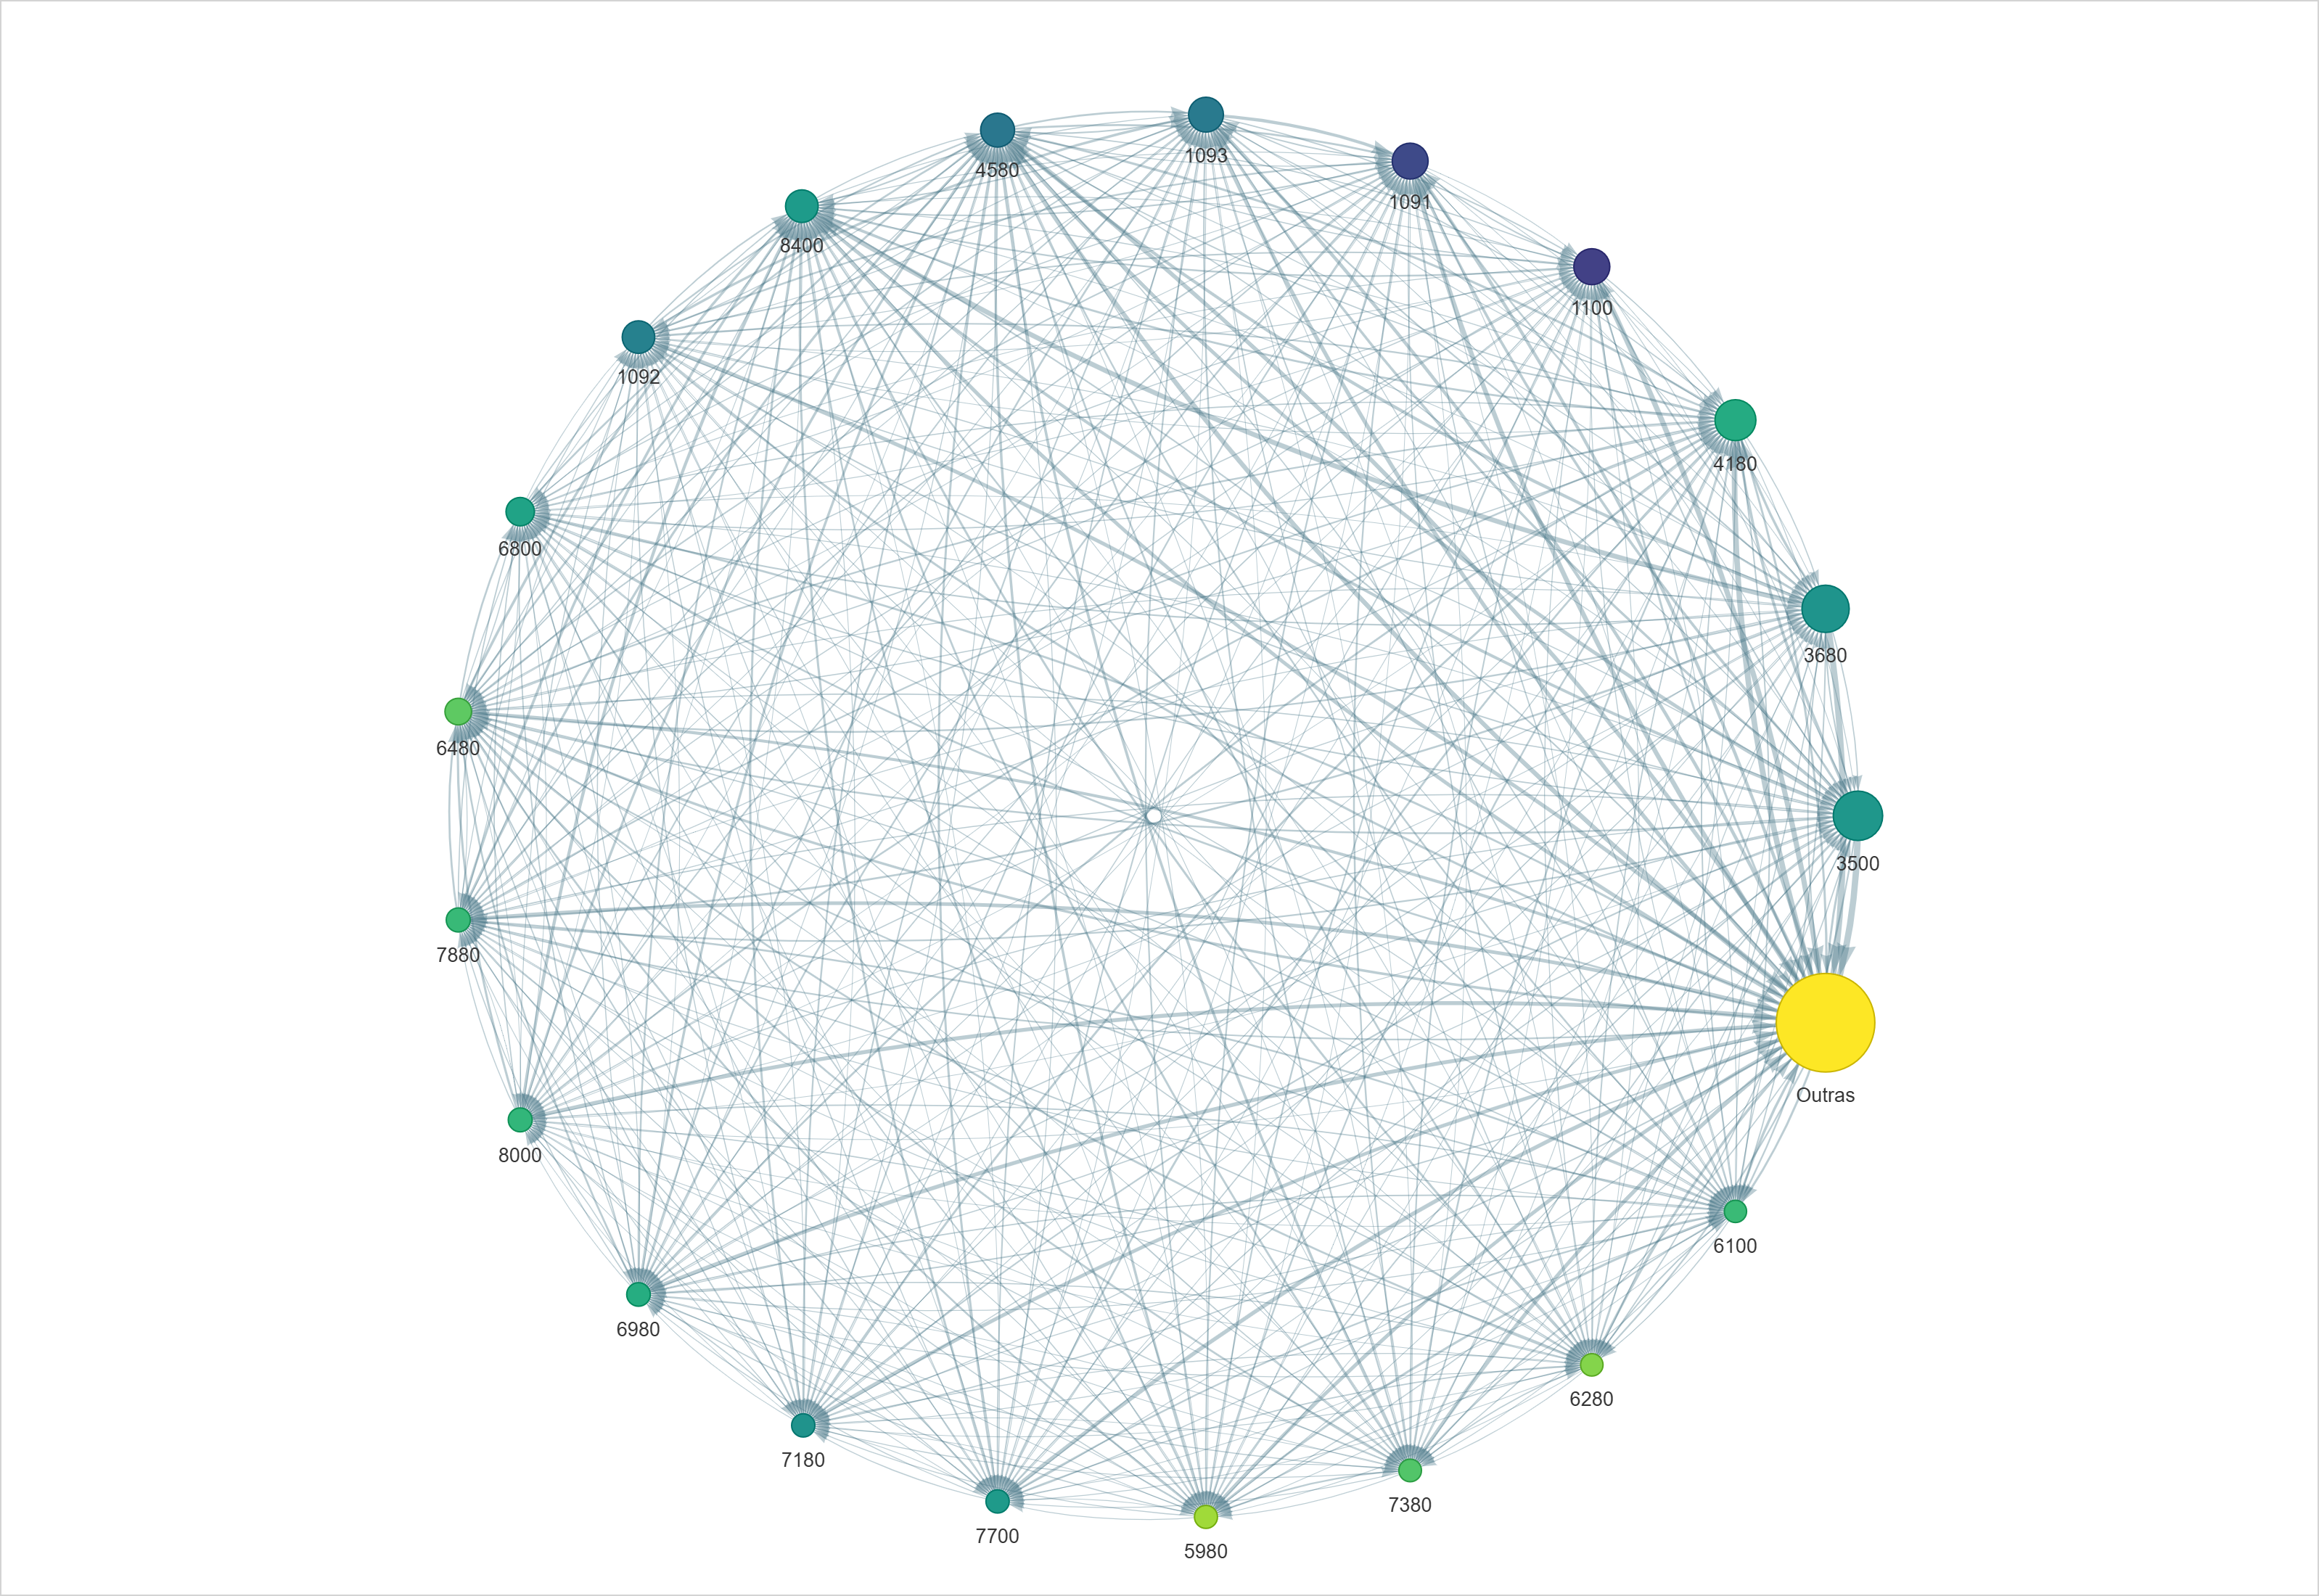
\includegraphics[width=\textwidth,height=0.87\textheight,keepaspectratio]{imagens/03_rede_circular.png}
\caption{Rede agregada em disposição circular. As 20 maiores emissoras são mantidas; as demais formam Outras. A área representa emissões próprias; a espessura, o peso da relação; a cor, a diversidade de destinos, crescente do roxo ao amarelo. As setas indicam os destinos da demanda final.}
\end{figure}

\clearpage
\begin{figure}[p]
\centering
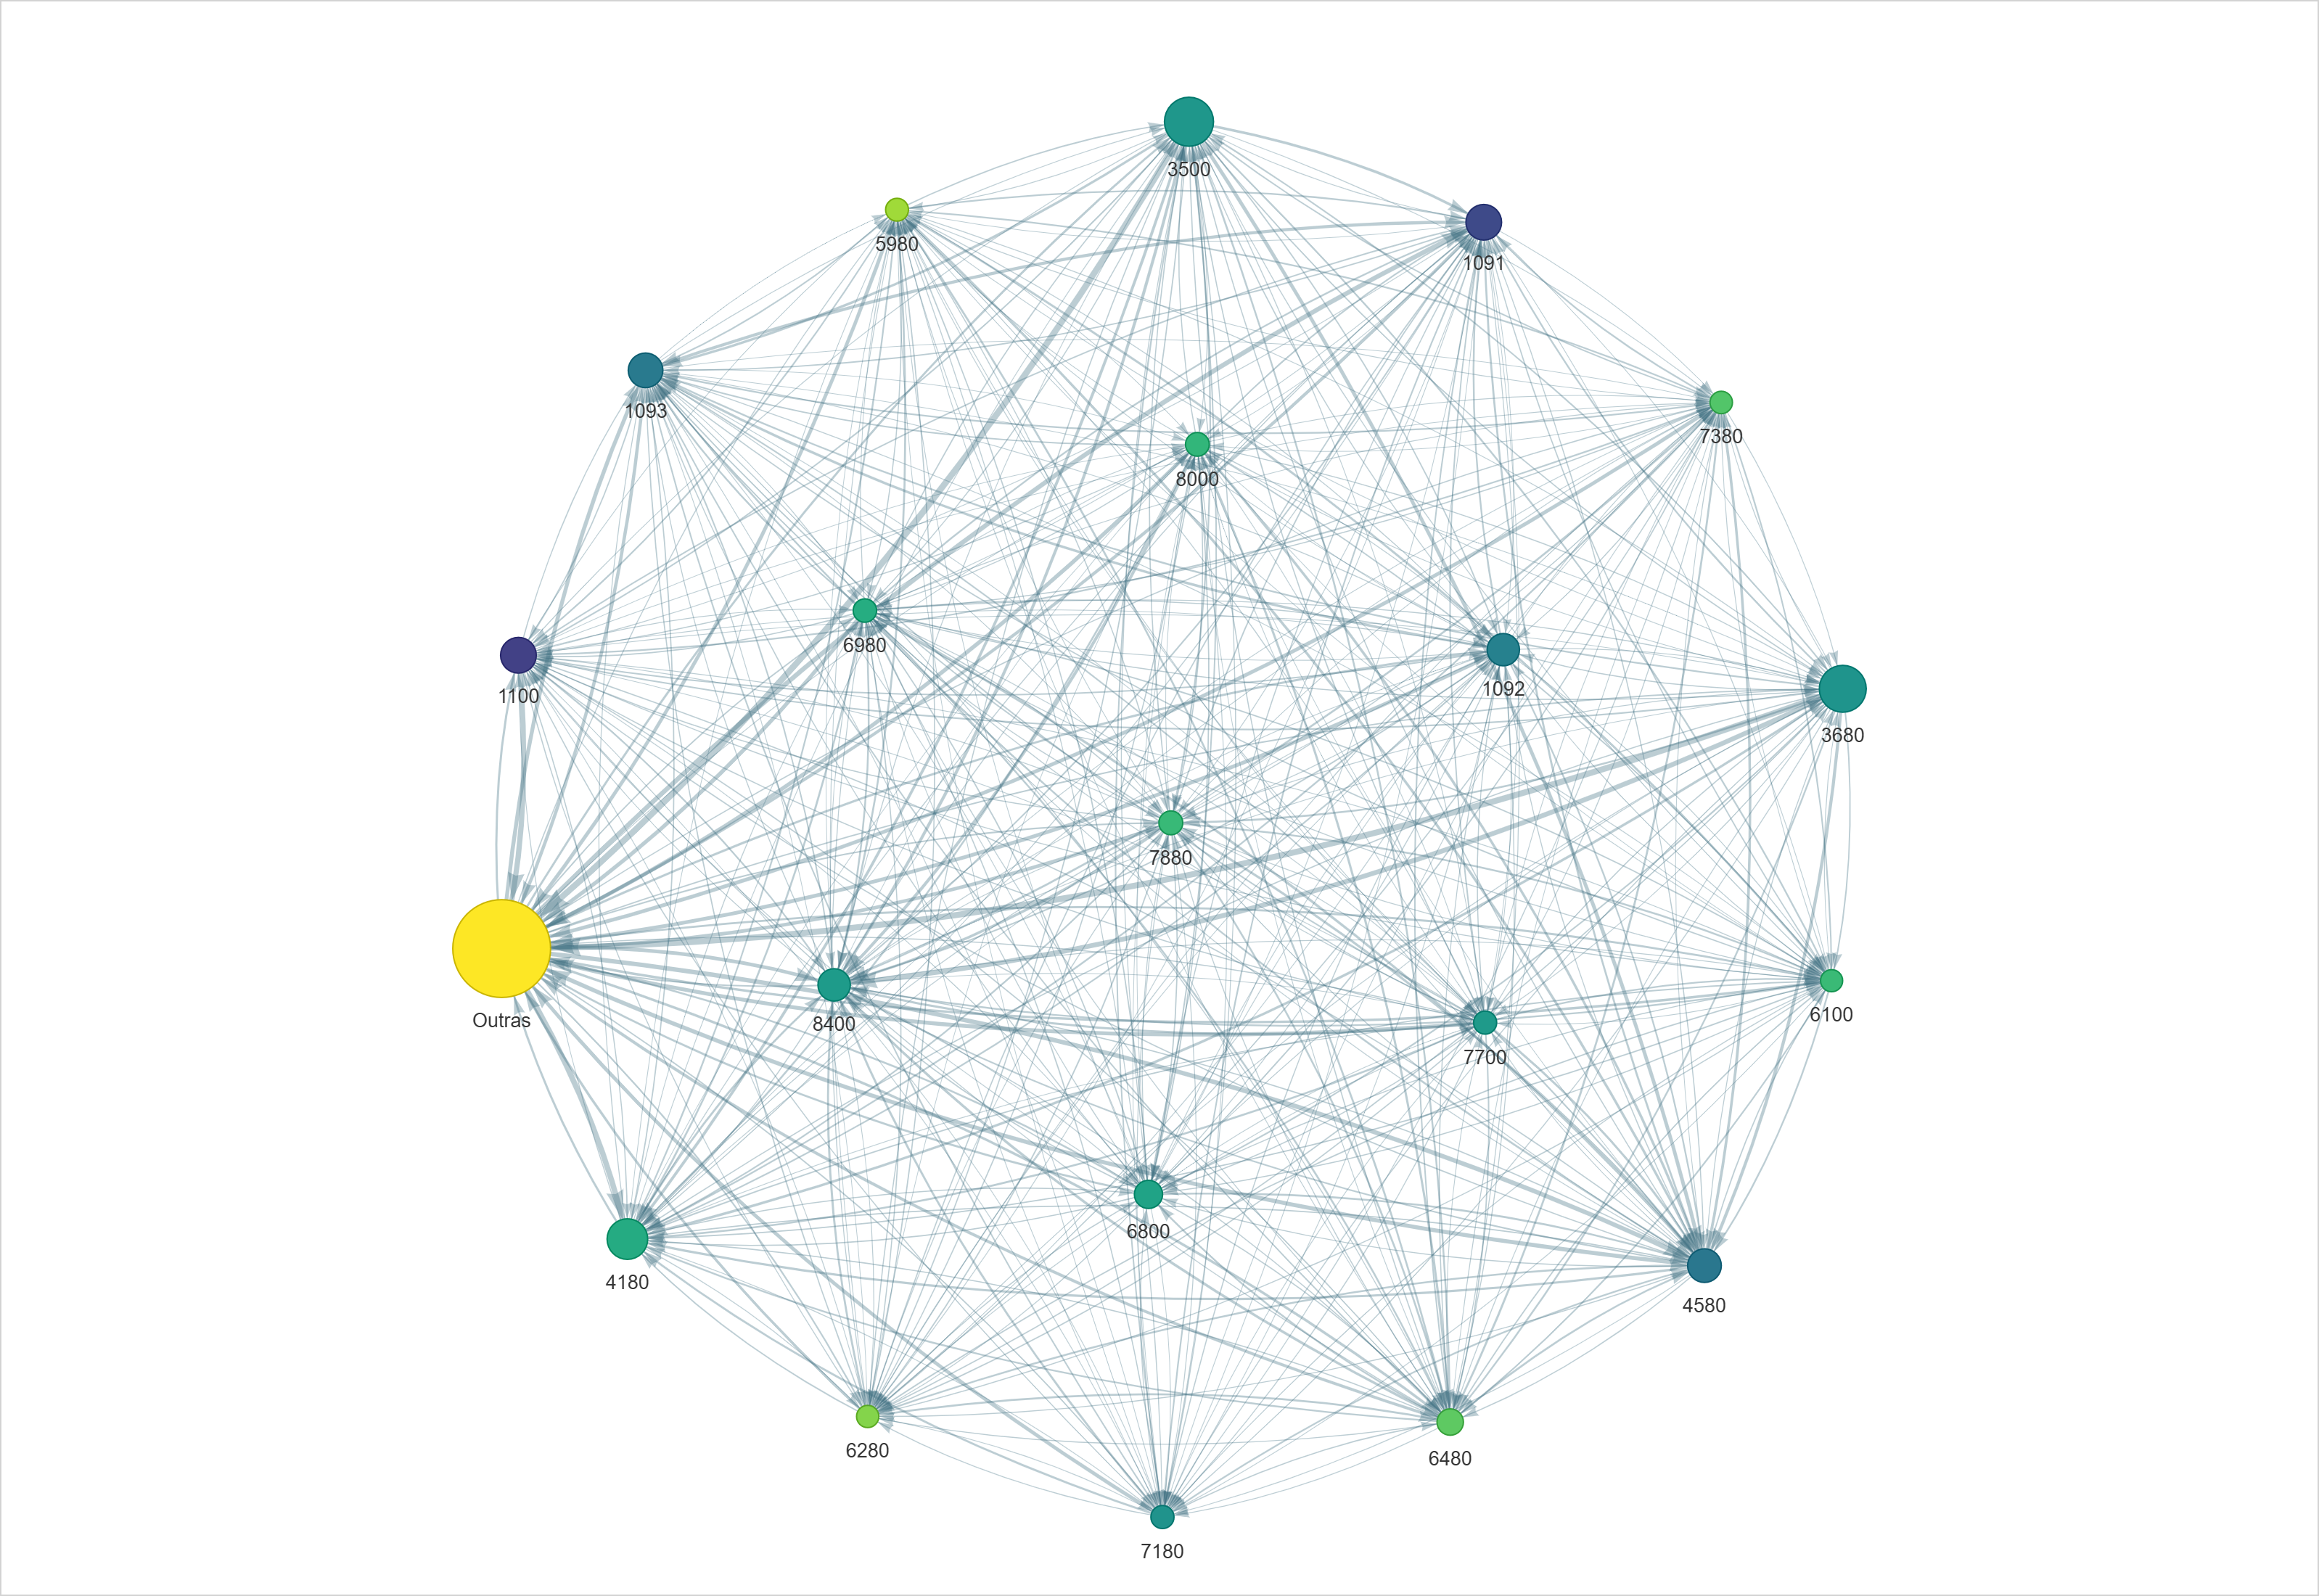
\includegraphics[width=\textwidth,height=0.87\textheight,keepaspectratio]{imagens/04_rede_forcas.png}
\caption{Rede agregada em disposição por forças. São os mesmos nós, pesos e escalas da figura anterior. A posição não representa distância econômica. As relações incluem requisitos diretos e indiretos; caminhos no desenho não são etapas físicas adicionais da produção.}
\end{figure}

\clearpage
\section*{Referências}
\begin{enumerate}
\item \textbf{Armstrong McKay, D. I. et al. (2022).} \href{https://doi.org/10.1126/science.abn7950}{\textit{Exceeding 1.5°C global warming could trigger multiple climate tipping points}}. \textit{Science}, 377, eabn7950.

\item \textbf{IBGE.} \href{https://www.ibge.gov.br/estatisticas/economicas/contas-nacionais/9085-matriz-de-insumo-produto.html}{\textit{Matriz de Insumo-Produto: Brasil, 2015}}.

\item \textbf{Marques, A.; Rodrigues, J.; Lenzen, M.; Domingos, T. (2012).} \href{https://doi.org/10.1016/j.ecolecon.2012.09.010}{\textit{Income-based environmental responsibility}}. \textit{Ecological Economics}, 84, 57–65.

\item \textbf{Miller, R. E.; Blair, P. D. (2009).} \href{https://doi.org/10.1017/CBO9780511626982}{\textit{Input–Output Analysis: Foundations and Extensions}}. 2ª ed. Cambridge University Press.

\item \textbf{Montoya, M. A.; Bertussi, L. A. S.; Allegretti, G.; Talamini, E. (2026).} \href{https://doi.org/10.1007/s10668-024-05251-8}{\textit{Brazilian energy and carbon footprints: structural changes and sectoral contributions to climate change}}. \textit{Environment, Development and Sustainability}, 28, 6725–6755.

\item \textbf{Rissman, J. et al. (2020).} \href{https://doi.org/10.1016/j.apenergy.2020.114848}{\textit{Technologies and policies to decarbonize global industry: Review and assessment of mitigation drivers through 2070}}. \textit{Applied Energy}, 266, 114848.

\item \textbf{Sanguinet, E. R.; Azzoni, C. R. (2024).} \href{https://doi.org/10.1016/j.rspp.2024.100015}{\textit{Carbon emissions drivers in Brazilian regional production chains: Value-added and consumption-based approaches}}. \textit{Regional Science Policy \& Practice}, 16, 100015.

\item \textbf{UNFCCC (2008).} \href{https://unfccc.int/resource/docs/publications/08_unfccc_kp_ref_manual.pdf}{\textit{Kyoto Protocol reference manual on accounting of emissions and assigned amount}}. United Nations Framework Convention on Climate Change.

\end{enumerate}
\end{document}
